\chapter{Design}

\section{Use case: Skriv besked}

\begin{figure}[h]
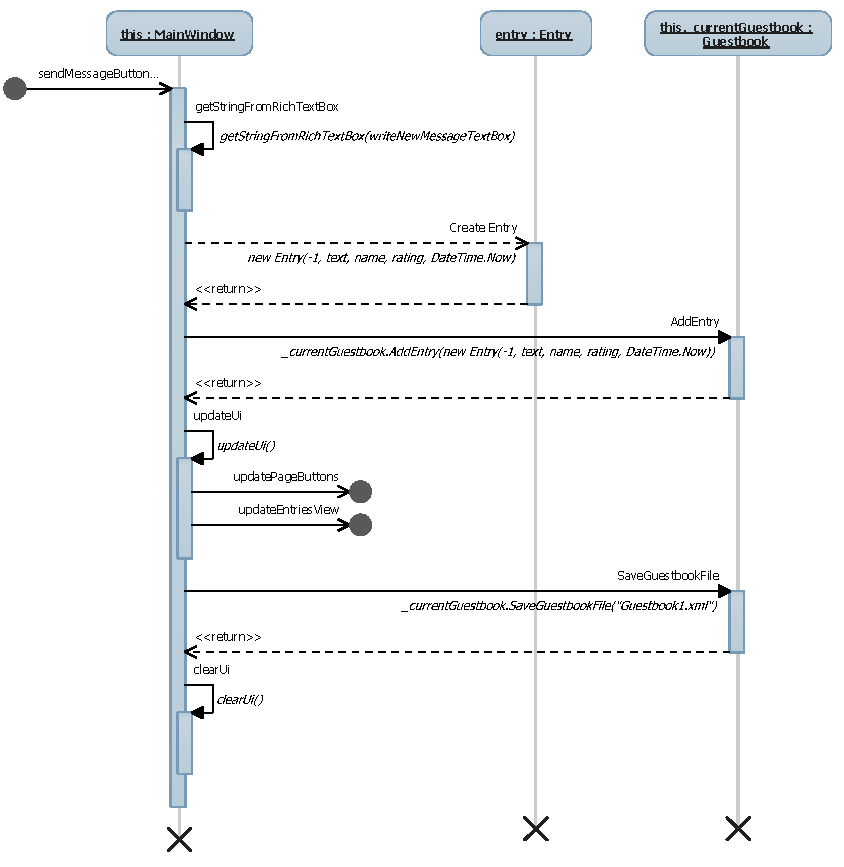
\includegraphics[width=\linewidth]{./add-entry-ssd}
\caption{Systemsekvensdiagram for AddEntry}
\label{add-entry-ssd}
\end{figure}
 
\begin{figure}[h]
\caption{Operationskontrakt for AddEntry}
\begin{itemize}
\item[]
\item[] \textbf{Use-case:} Skriv en besked til g�stebogen
\item[] \textbf{Operation:} Tilf�j besked (navn, besked: String, vurdering: Int, dato: Date)
\item[] \textbf{Pre:} Navn, vurdering og besked er udfyldt
\item[] \textbf{Post:} Beskeden er tilf�jet
\item[] \textbf{Output:} "Beskeden er tilf�jet"
\end{itemize}
\end{figure}

\section{Use case: Skjul besked}

\begin{figure}[h]
\caption{Operationskontrakt for HideEntry}
\begin{itemize}
\item[]
\item[] \textbf{Use-case:} Administratoren skjuler en besked i g�stebogen
\item[] \textbf{Operation:}  Skjul besked (navn, besked: String, vurdering: Int, dato: Date)
\item[] \textbf{Pre:} Beskeden er valgt 
\item[] \textbf{Post:} Beskeden er skjult.
\item[] \textbf{Output:} Beskeden er nu blivet skjult.
\end{itemize}
\end{figure}

\section{Use case: Slet besked}

\begin{figure}[h]
\caption{Operationskontrakt for DeleteEntry}
\begin{itemize}
\item[]
\item[] \textbf{Use-case:} Administrator sletter en besked fra g�stebogen
\item[] \textbf{Operation:} Slet den valgte besked (navn, besked: String, id, vurdering: Int, dato: Date)
\item[] \textbf{Pre:} Der er valgt en besked
\item[] \textbf{Post:} Den valgte besked bliver slettet fra g�stebogen
\item[] \textbf{Output:} "Beskeden er slettet"
\end{itemize}
\end{figure}

\section{Use case: Skift g�stebog}

\begin{figure}[h]
\caption{Operationskontrakt for ChangeGuestbook}
\begin{itemize}
\item[]
\item[] \textbf{Use-case:} Administratoren v�lger hvilken g�stebog der er aktuelt vist for brugeren
\item[] \textbf{Operation:} �ndre g�stebogen (G�stebog: Guestbook).
\item[] \textbf{Pre:} Den aktuelle g�stebog er valgt
\item[] \textbf{Post:} G�stenbogen er blevet valgt.
\item[] \textbf{Output:} Du har nu valgt en ny g�stebog
\end{itemize}
\end{figure}